\scanpage{21}
\margin{20}

\figure{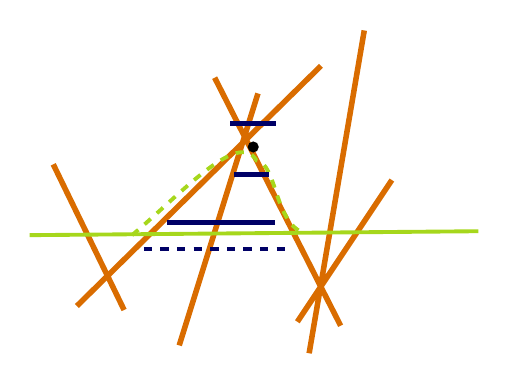
\begin{tikzpicture}[x=1cm,y=1cm]
\draw[orange!85!black,line width=2pt] (-1.4,-.9)--(1.7,2.15) (-1.7,.9)--(-.8,-.95) (-.1,-1.4)--(.9,1.8) (.35,2)--(1.95,-1.15) (1.55,-1.5)--(2.25,2.6) (1.4,-1.1)--(2.6,.7);
\draw[yellow!65!green,line width=1.4pt] (-2,0)--(3.7,.05);
\draw[yellow!65!green,line width=1.4pt,dashed] (-.7,0)..controls(-.1,.5)and(.65,1.35)..(.88,.95)..controls(1.15,.9)and(1.1,.15)..(1.5,.02);
\draw[blue!40!black,line width=1.6pt] (-.25,.16)--(1.12,.16) (.55,1.42)--(1.13,1.42) (.6,.77)--(1.04,.77);
\draw[blue!40!black,line width=1.4pt,dashed] (-.55,-.18)--(1.3,-.18);
\fill (.84,1.12) circle (2pt);
\end{tikzpicture}}

{\ttfamily\begin{tabular}{l}
\unsure{********************************************************************************}\\
*JESNEWS DU \unsure{03/08/1982|30/08/1982} C68 CADARACHE *\\
\unsure{********************************************************************************}\\
* DEPUIS LE 1/7/82 LES ALIAS DES COMMANDES LIBRARIAN *\\
* LIBGET (LG) ET LIBSAVE (LS) SONT SUPPRIMES, *\\
* POUR EVITER UNE POSSIBILITE DE CONFLIT AVEC *\\
* LE MEME ALIAS DES COMMANDES STANDARD IBM. *\\
* ******** *\\
* ATTENTION *\\
* MISE EN SERVICE LE VENDREDI 30/7/82 A 9H00 DE LA DEUXIEME PHASE DE GAF *\\
* SUR 168 CADARACHE. *\\
* ELLE PERMET D'UTILISER DANS LA CDE. KEEP TSO ET DANS LA PROCEDURE KEEP *\\
* BATCH UNE POSSIBILITE D'AFFECTATION DE TYPE DE SAUVEGARDE AU NIVEAU DU *\\
* FICHIER.CETTE POSSIBILITE EST VIVEMENT CONSEILLEE. *\\
* POUR PLUS AMPLES INFORMATIONS VOIR NOTE TECHNIQUE CISI MVS140,LA NOTE *\\
* MVS 145 ETANT SUPPRIMEE. *\\
* *\\
* EXEMPLES D'UTILISATION: *\\
* *\\
* BATCH: DSN=NOM.DU.FICHIER.A.SAUVEGARDER,DELAY=TYPE DE SAUVEGARDE *\\
* *\\
* TSO: *\\
* K DA('NOM DU FICHIER A SAUVEGARDER') DELAY(TYPE DE SAUVEGARDE) *\\
* *\\
* TYPES DE SAUVEGARDE: *\\
* *\\
* W SAUVEGARDE HEBDO. *\\
* D SAUVEGARDE JOURNALIERE. *\\
* NOS SAUVEGARDE MENSUELLE. *\\
* * PARAMETRE PAR DEFAUT. *\\
* *\\
\unsure{********************************************************************************}
\end{tabular}}

{\ttfamily\begin{tabular}{l}
\unsure{*******************************************************************}\\
* *\\
* - J E S N E W S F R 1 - LE 16/08/82 *\\
* *\\
*-----------------------------------------------------------------*\\
* *\\
* DEPUIS LE LUNDI 12 JUILLET 82, LES CLASSES DE TRAVAUX D ET E *\\
* SERONT ETENDUES POUR UNE TAILLE MEMOIRE SUPERIEURE A 1024 K *\\
* SE REPORTER A LA NOTE TECHNIQUE MVS141. *\\
* *\\
*-----------------------------------------------------------------*\\
* A PARTIR DU LUNDI 9 AOUT 1982, IL SERA POSSIBLE D'IMPRIMER *\\
* SUR XEROX 9700 (DESTINATION SAC) DES FICHIERS UTILISANT LE *\\
* COUPLE DE JEUX DE CARACTERES : (GS15,GT15) *\\
* *\\
*-----------------------------------------------------------------*\\
* *\\
* LE 16/08/82 : *\\
*------------- *\\
* -LE 370/168 SERA ARRETE DU VENDREDI 20 AOUT A 19H JUSQU'AU *\\
* LUNDI 23 AOUT A 8H.( MISE A NIVEAU TECHNIQUE.). *\\
* *\\
\unsure{*******************************************************************}
\end{tabular}}
